\documentclass[a4paper,12pt]{article}
\usepackage{a4}
% \usepackage{isolatin1}
\usepackage[utf8]{inputenc}
\usepackage[T1]{fontenc}
\usepackage[pdftex]{graphics}
\usepackage{graphicx}
\usepackage{subfig}
\usepackage{color}
\usepackage{amsmath,amsthm,amstext,amssymb,amscd}
\usepackage{url}

\newcommand{\name}[1]{\textsc{#1}}
\newcommand{\codename}[1]{\texttt{\small #1}}

\newcommand{\mf}{\name{MathletFactory }}
\newcommand{\mumie}{\name{Mumie }}
\newcommand{\nc}{\name{number class }}
\newcommand{\mo}{\name{M-Object }}
\newcommand{\mos}{\name{M-Objects }}
\newcommand{\mmo}{\name{MM-Object }}
\newcommand{\mmos}{\name{MM-Objects }}
\newcommand{\cp}{\codename{ControlPanel }}
\newcommand{\formlang}{\name{formal language }}
\newcommand{\oorange}{\name{Oorange }}

\hyphenation{ma-the-ma-ti-cal}

\begin{document}

\begin{titlepage}
\begin{center}

\vspace*{1.5cm}

\LARGE{\textbf{The Mumie}}\\
\huge{\textbf{MathletFactory}}\\[0.5cm]---\\[0.5cm]

\Large{An Open Source Java Library for Interactive \\Mathematical Applets (\textit{``Mathlets''})}\\[1.5cm]

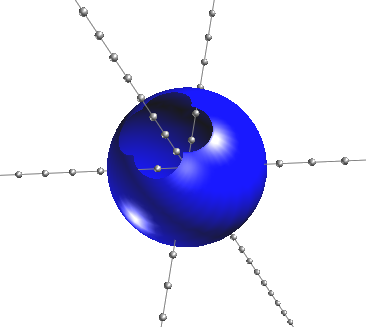
\includegraphics[scale=0.9]{images/front.png}

\vspace*{1.5cm}

\emph{Author:}\\
Markus \textsc{Gronau}\\[0.3cm]
\today

\end{center}
\end{titlepage}

\newpage

\parindent = 0cm

\vspace*{3.0cm}

Copright 2008 Integral Learning GmbH. All rights reserved.\\
Documentation is provided ``as is'' and may not be reproduced or copied without permission.
Information contained in this document is without any warranty for correctness.\\
\\
%\vfill
%\hrule
%\vspace{0.3cm}
The picture on the front page was taken from a screenshot of the mathlet \codename{SurfaceInR3} and shows
a parameterized surface in $\mathbb{R}^3$.

\newpage

\tableofcontents 

\newpage

\section{Abstract}

\subsection{About this Document}

This document reports on the \mumie \mf (versions 2.0 and 2.1), an  open-source Java library for interactive mathematical applets.
This document gives a structural overview of the main features but does not intend to describe in detail the
neccessarities for building own programs. These information are rather contained in the \mf \textit{tutorial}.\\
Some of the mentioned features are only available in the milestone release 2.1.

\subsection{About the Mumie MathletFactory}
The \mumie is an e-learning platform specialized in mathematics and mathematical sciences.
It is a fully web-based learning- and teaching environment using standard techniques
(such as XHTML, MathML and Java) for deploying mathematical content to the end-user inside 
a standard compliant internet browser.\\
\\
The \mf is a Java library and part of the \mumie in which it is used to produce and to visualize
dynamic, interactive mathematical content with Java applets (so called ``mathlets''). It allows
the rapid development of such mathlets, containing complex mathematical algorithms and scenes
along with a common generic behaviour and appearance.\\
The \mf library contains a large collection of mathematical objects (so called \mmos), which can 
be used both in calculations and presentations of dynamic problems.
Their visualizations may be both symbolic and graphical (both 2D and 3D).
Their state may be interactively changeable by the user and may cause further interaction between them.\\
\\
The \mf is developed since 2001 and released in 2007 the milestone 2.0, which has been used since then by
several thousands of students at different international universities. The main development
effort is actually done for the milestone 2.1 which will be released in spring 2008.\\
\\
The \mf library is open source and provided under the MIT license. It is compliant with 
all Java versions of SUN Microsystems and Apple Inc. starting with Version 1.4.2\footnote{Some 
additional extensions may require a newer Java version.}. Further information and documentation 
as well as source code is available under \url{http://www.mumie.net}.


\newpage

\subsection{Fundamental Concepts}

\subsubsection*{Generic programming of mathlets}
The programming of mathlets is generic and easy to use but does not restrict the applet developer
in his creativity. By automatically adding standard features to new mathlets and providing a
flexible and generic applet ``skeleton'' the developer can concentrate on the mathematical content.\\
The \mf library acts hereby as a reusable component system.

\subsubsection*{Separation of logic and representation}
The \mf follows the philosophy to separate the (abstract) mathematical object from its further
representation(s) on the screen, defining a veritable Model-View-Controller architecture (MVC).
By handling interactive actions (e.g. user interaction) through generic but specific \textit{events}, 
changes are automatically reflected to the mathematical model and also propagated to any dependant 
objects, allowing even complex dependency trees.

\subsubsection*{Abstract number fields for arbitrary-precise calculations}
Most mathematical objects are based on an abstract number class which makes it possible to perform
calculations on a particular number field with its own arbitrary precision. While some operations
need a complex number field, other situations can be more satisfied with an answer in whole numbers.
Furthermore while e.g. floating point operations are executed faster than rational ones, the latter 
are more precise and user friendly.

\subsubsection*{Open extensible framework}
The \mf library offers a wide spectrum of objects for the most needed mathematical entities and 
applet developer's concerns but also can be extended in almost every included technology\footnote{
Some extension features are only available in the up-coming milestone 2.1}. By
providing an open framework and both a complete API documentation and tutorials for its techniques, 
the \mf truly underlines its open source idea.


\textheight = 670pt
\newpage
\footskip = 0pt

\section{Applet Skeleton Framework}

With providing a flexible and powerful ``skeleton'' framework for applets, the developer has neither to
``reinvent the wheel again'', nor to transfer whole passages of code for new programs. Instead, basing
on an applet skeleton, mathlets have a generic interface for both the code itself and the placement of
code. This simplifies the understanding of mathlet code (even if it is not the ``own'' code) and thus
reduces developing and debugging time.

\subsection{Mathlet Instance Methods}

Observing the life cycle of Java applets, these offer several \textit{entry points} for actions to take
place according to the current applet's \textit{state}. One of these is the \codename{init()} method which 
will be called after the applet class is initialized. Observe that many applet specific features are not
available till the \codename{init()} method of the applet is reached. Calling this method is necessary for 
properly initializing the mathlet's runtime, subclassing applets must be aware of this.
Since every mathlet extends one of the skeleton classes, every feature can be easily accessed via one
of the mathlet's instance methods but only after the runtime's initialization.

\begin{figure}[h]
  \begin{center}
    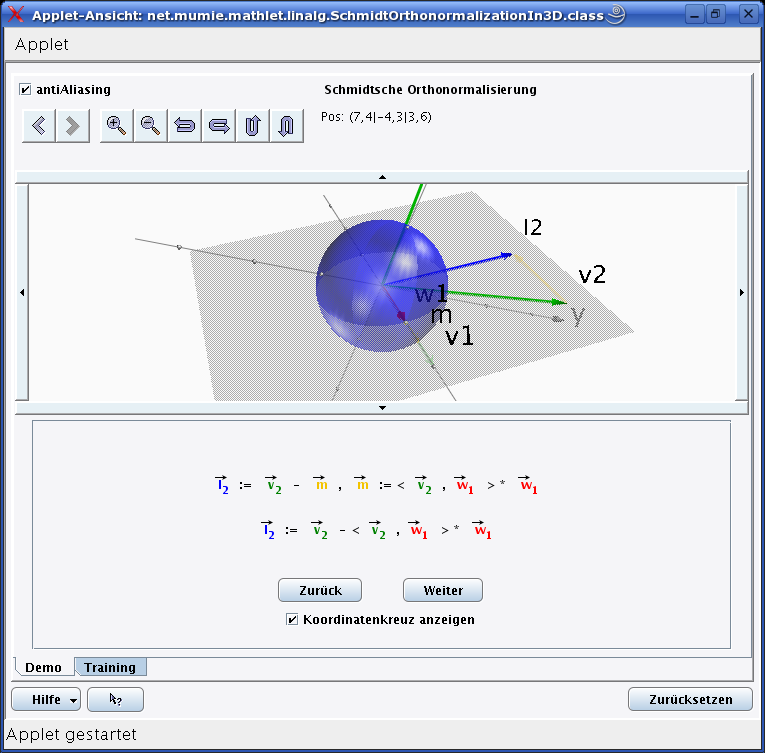
\includegraphics[height=12cm]
      {images/screenshot_schmidt_orthonormalization.png}
    \caption{Screenshot: Schmidt Orthonormalization}
  \end{center}
\end{figure}

\textheight = 621pt
\newpage
\footskip = 30pt

\subsection{User Interface}

Creating user interfaces in Java can be a very complex task: on the one hand code can become very large
for even simple interfaces, thus making it hard to maintain it. On the other hand a common appearance
with a distinctive design across all programs is wanted. These implications were resolved in two ways:
first by providing basic layout templates which can be used as a fundament for new mathlets and secondly
with powerful layout techniques which allow to arrange components in a ``text editor like'' manner and 
thus permitting a ``human readable'' and very short layouting code without a long training period into
Java SWING or the \mf library.\\

\subsubsection*{Skeleton Templates}

Every mathlet's layout defines three basic parts: the title, the content and (bottom) button area.
The different skeleton classes only differ in the content area, which may include one or more
graphical drawing boards (each a 2D or 3D \name{canvas}) or none. All of them include the functionality 
of an integrated \cp to display symbolic and descriptive content underneath the canvas/canvi.\\
The fundamental skeleton class of all further template classes is \codename{BaseApplet} and may also be used
as a basis (i.e. super class) for own applets.

\subsubsection*{Laying out Control Elements and Text}

Each mathlet defines a single \cp but may also use several of them, even nested into each other.
Content in a \cp is arranged in a text editor like manner i.e. into rows. Each row alignes its content
from the left to the right and can have its own horizontal alignment. Inserting a \textit{line break}
causes the current line to end and to start a new line which will be used for the further adding of 
components: \codename{insertLineBreak()}.\\
Adding text can be achieved via \codename{addText(String text)} or with one of the \codename{addText} methods
requesting an additional color and/or font argument.

\subsubsection*{Entering Descriptive Content}

Descriptive texts beside mathematical formulas are essential inside an educational program like mathlets.
For this purpose, three common text ``formats'' are available: TeX, HTML and plain text. Each format 
can be used in any text component and offers different advantages compared to the other two.

\textheight = 650pt
\newpage
\footskip = 0pt

\subsubsection*{Common Baseline Sharing}

As the bridge between textual and symbolic content, every UI component supports a common baseline sharing
with all other elements aligned in the same row (e.g. inside a \cp or a text viewer). This technique
allows an ordered and clearly arranged layout of e.g. mathematical formulas surrounded by descriptive
text blocks.

\subsection{Multilinguality}

Every language sensitive component inside the \mf library uses the \name{messages} technology which 
allows to combine an abstract \textit{message key} with a concrete translation (the real \textit{message})
during execution time. By this way no programming code must contain any language dependant expressions,
thus permitting to maintain any descriptive content beside the source code and to add translations for 
new languages for already existing features.\\
New messages can be defined as stated in the \textit{Java Property Format} specification in a 
\texttt{key = value} notation in a file named \texttt{Messages\_[LANG].properties} where [LANG] means 
the language's code. They can be retrieved inside a mathlet with the instance method 
\codename{getMessage(String key)}.

\begin{figure}[h]
  \begin{center}
    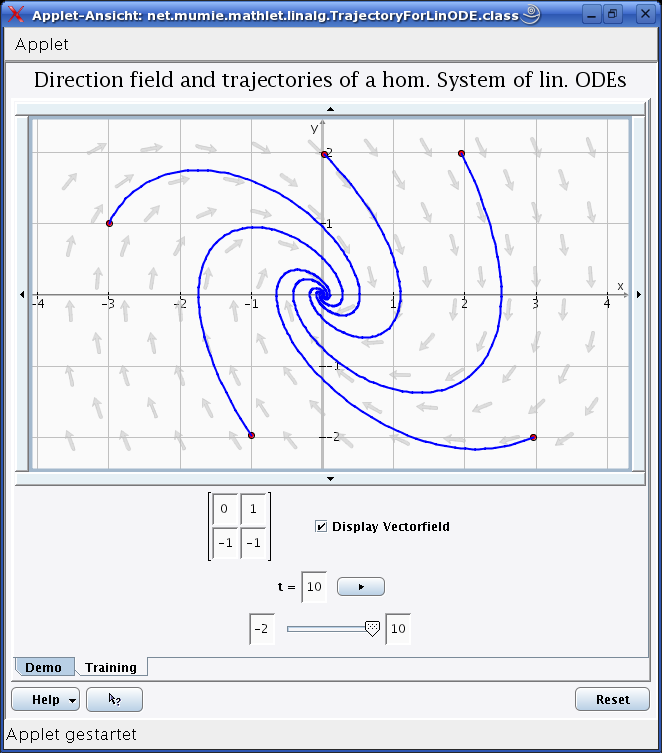
\includegraphics[height=10.5cm]
      {images/screenshot_trajectory_linODE}
    \caption{Screenshot: Trajectories for a Linear Ordinary Equation System}
  \end{center}
\end{figure}

\textheight = 621pt
\newpage
\footskip = 30pt

\subsection{Help System}

The \mf supports two types of help systems: if the \name{JavaHelp} extension is available, the (default)
help system can be used providing various standard features like HTML and print support, a navigatable 
table of contents or a context sensitive help. If the default help system cannot be used for any reasons
a simpler built-in system will be loaded instead, permitting a less confortable but sufficient help.\\
Like all language sensitive technologies, both help systems respect the mathlet's language setting and
may be extended for new languages but also with additional help topics.

\subsection{Error Handling}

Due to the complexity of software systems and their configurations (including the internet browser and the 
\textit{Java Plug-In}) a flawless program execution cannot be assured, even if the system can be
declared as \textit{stable}. These \textit{runtime errors} may be caused by unpredicted user actions,
defective network connections, faulty configured systems or simply software bugs and should be catched
and processed by an appropriate error handling system, which notifies the user and proposes useful solutions
for the problem. While Java applets always run on the client side, an error report describing the failure
and including system information may be useful for further debugging and bug fixing procedures of the
administrating staff.\\
For this purpose the \mf includes a complete quality feedback system with automatical generating
error reports, which can be viewed and probably sent to a \mumie server by the user.\\
At this point, based on the experiences with error reports from students, the \mf is able to use some 
workarounds and bug fixes for various incompatibilities between the multiple Java versions and vendors.

\subsection{Common appearance}

Per default every mathlet uses an elaborated theme (the \codename{MumieTheme}) for the 
\textit{Java Metal Look\&Feel} which assures a common appearance across all operating systems and Java
versions/vendors and updates the default Java theme with a clearer and more modern look.
This theme allows a scalable appearance for all mathlets including color, font and other \textit{look and feel} 
relavant settings.


\newpage

\section{Model-View-Controller Architecture}

The \mf holds on the paradigm to separate the logic from its representation on the screen, thus
introducing various \textit{interfaces} between the single technologies. These interfaces guarantee an 
implementation of new features which is independant of restrictions of already exisiting components.
Hence this ``Model-View-Controller'' architecture simplifies the creation of new mathematical objects and
allows a clear distinction between the mathematical \textit{model}, the \textit{view} on the screen and 
the \textit{controller} processing user actions and updating the model.\\
See figure \ref{fig:mvc_common} for an overview of the components in such an architecture.

\begin{figure}[h]
  \begin{center}
    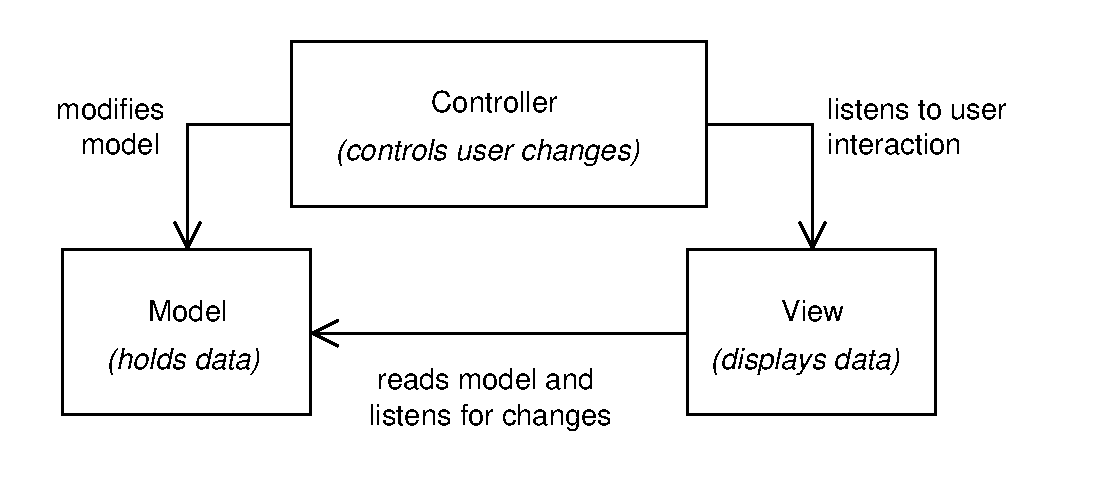
\includegraphics[width=10cm]
      {images/mvc_common.pdf}
    \caption{Common role allocation in a MVC architecture}
    \label{fig:mvc_common}
  \end{center}
\end{figure}

\subsection{Model Architecture}

In the \mf there are two \textit{grades} of models: first the pure mathematical model describing the internal
state of a mathematical entity/object (the \name{M-Object}) and secondly the extending \textit{multimedial} 
model containing additional \textit{display properties} and interfaces for the MVC architecture (the \mmo).

\subsubsection*{Mathematical Models}

A mathematical model or a \mo holds the internal data of an entity and offers methods for operating with it.
\mos are completely detached of any viewing and interaction capabilities, thus forming a \textit{calculation layer}.\\
They are usually based on an abstract \nc which is used to interchange number values with other \mos and 
to execute primitive calculations (see section \ref{subsection:arithmetic_model}).

The \mo interface was deliberately designed as an \textit{open interface} thus a \mo is free of any restrictions.


\subsubsection*{MM-Objects}

\mmos are both mathematical and multimedial components and are the primary entities with which a developer 
has to deal with. They typically extend a \mo and add the \mmo capabilities via interfaces\footnote{due to the 
fact that multiple inheritance is not possible in Java}, thus forming an \textit{interactivity layer}.

Some \mmos incorporate their mathematical model for simplicity.

\vspace{1.0cm}

\subsection{View Architecture}

The view of a \mmo is its representation drawn on the screen which is performed by a \textit{drawable}.
The drawable's data is transformed from the mathematical model to a display model via a \textit{transformer}.
Using an abstraction layer between these two models allows different abstract presentations of the same
mathematical content.

\subsubsection*{Transformers}

A transformer is responsible for the correct adjustment of drawables depending on the current \name{MM-Objects}'s
state. Every time a \mmo needs to be rendered, the transformer's \codename{render()} method will be called,
allowing to update the display model and the view(s).\\
A transformers is qualified by the master's type (i.e. the \name{MM-Objects}'s type), a screen type 
(e.g. 2D, 3D, ``no canvas'' for symbolic views) and a transform type, which describes the transform
into the display model. Every \mmo defines a default transform type for both symbolic and graphical representations.\\
The base class of all transformers is \codename{GeneralTransformer} which is also responsible for registering
the transformer mappings and creating the appropriate transformer instances on demand.

\subsubsection*{Drawables}

``Drawable'' is the abstract name of a viewing component, which itself can composed by various 
\textit{canvas drawables} for graphical views or by \textit{container drawables} for symbolic views.
Drawables are created and updated by transformers and are designed to be reusable in new representations.


\newpage

\subsection{Controller Architecture}

The controller architecture differentiates between actions in a canvas and those in a SWING container.
The later use a different, easier technique since container drawables can only be edited on one way: with
the keyboard. A canvas instead,  when encountering an user action, propagates it to its 
\textit{canvas controller} who generates a corresponding \codename{MMEvent} and notifies the appropriate 
handler dealing with this action. These modify the \mmo and invoke an update of dependant objects, which
is done by \textit{updaters}.
Actions can originate from the mouse and/or the keyboard.


\subsubsection*{Handlers}

Handlers track mouse or keyboard actions (or a combination of both) in canvas drawables and react
accordingly. Each handler is characterized by a \codename{MMEvent} which describes an action the handler 
wants to deal with. There are two different types of handlers: object specific and global handlers.
The first are added to a \mmo and modify its internal state while the later are added directly to a canvas 
and transform the view of a scene.\\
The \mf contains a large number of predefined object specific handlers for the personal use.

\subsubsection*{Updaters}

Updaters track changes in dependant \mmos and adjust the \textit{slave} \mmo they were added to accordingly.
As the simplest implementation, the \codename{DependencyUpdater} allows to adjust \mmos by placing arbitrary 
code on-the-fly. Besides there is a large number of predefined updaters for the most common needs.

\subsubsection*{Events}

Events (or more precisely \codename{PropertyChangeEvents}) are used to inform the master \mmo about changes
in symbolic drawables. This is typically due to user interaction inside the SWING container where a
content string, describing the drawable's data, can be edited in a textfield. If the new input is
validated, an event is fired to the master \mmo which adjusts its internal state and propagates the
changes.


\newpage

\subsection{Architecture Overview}

The main components of the MVC architecture as well as their primary functions are:\\
\\
\begin{tabular}{ll}
  MM-Object & both mathematical and multimedial component \\
  Transformer & transforms mathematical model and updates drawable's view \\
  Drawable & visualizes the display model's content on the screen \\
  Handler & modifies mathematical model after mouse and/or keyboard action \\
  Updater & modifies slave \mmo after dependant \mmo has changed \\
\end{tabular}

\vspace{0.5cm}

The interaction between these components can be seen in the next figure which shows a simplified version,
reduced to one single representative for each component's type.

\begin{figure}[h]
  \begin{center}
    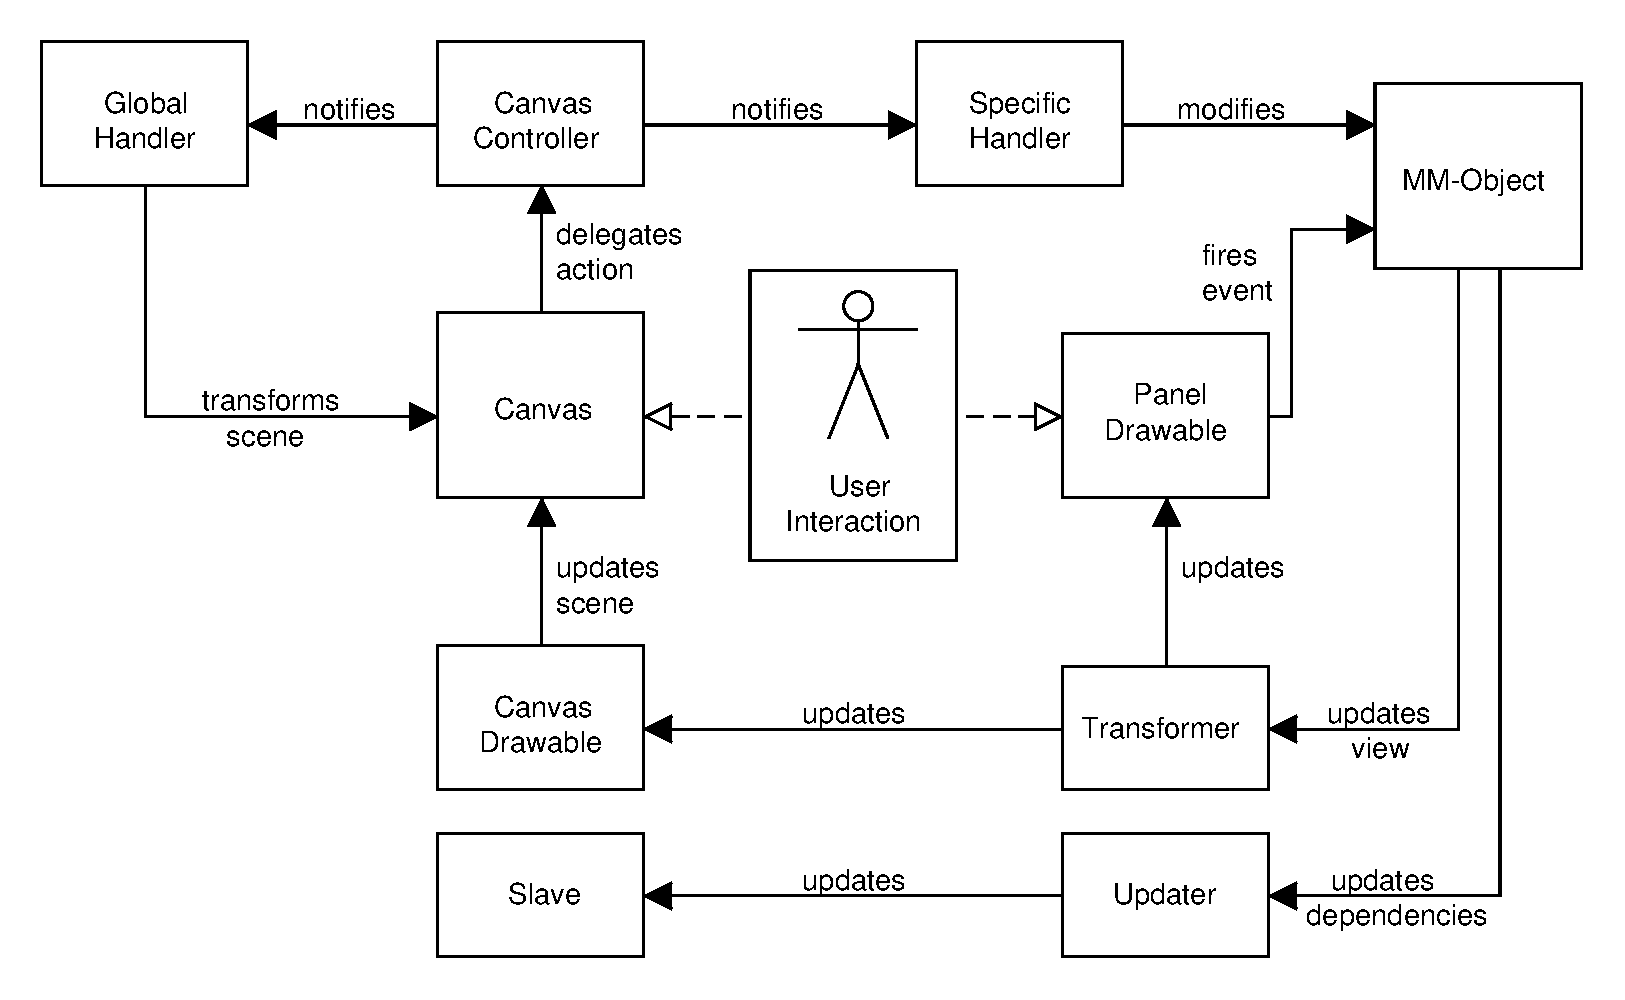
\includegraphics[width=14cm]
      {images/mvc.pdf}
    \caption{Interaction diagram of the MVC architecture}
    \label{img:mvc}
  \end{center}
\end{figure}

When the user modifies a graphical representation (e.g. drags a vector in a 2D canvas), the canvas propagates
the AWT event (e.g. mouse drag event) to its canvas controller who generates a corresponding \codename{MMEvent}
and searches for an object specific handler: First it checks if a canvas object currently owns the focus and if
such an object could handle the action. If one of these conditions is not met, the list of global handlers
will be searched for a responsible handler instead. When a valid handler is found, it is supposed to react 
to the event by adjusting the mathematical model accordingly.\\
If any updater is associated with the underlying \mmo its \codename{doUpdate()} method will be called, in
order to adjust the internal state of any dependant object which in turn might have other dependant objects
and so on. Once all required operations are finished, every out-dated view will be redrawn (both 
graphical and symbolic representations).
 
\vspace{1.0cm}

\begin{figure}[h]
  \begin{center}
    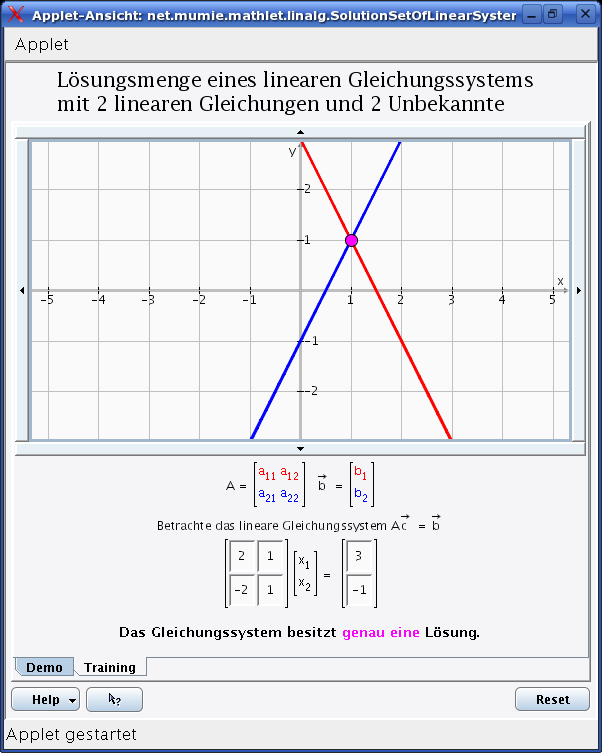
\includegraphics[height=14cm]
      {images/screenshot_solution_set.png}
    \caption{Screenshot: Solution Set of a Linear Equation System}
  \end{center}
\end{figure}

%\subsection{Graphical View Architecture}

%\subsection{Symbolic View Architecture}


\newpage

\section{Mathematical Models}

\subsection{Arithmetic Model}
\label{subsection:arithmetic_model}

Since number fields and their corresponding properties play a fundamental role in numerical calculations,
the \mf uses \textit{abstract arithmetics} for defining mathematical algorithms and properties and allows
therewith to treat them independently of any number field and its precision. By using e.g. a rational 
number field, the precision of calculations can be freed of rounding errors, a common mathematical 
problem in computer sciences.\\
This technique is based on an abstract \nc (\codename{MNumber}) which defines primitive arithmetic operations 
on an abstract number field.\\
The dependence of an abstract number field can be expressed by the interface \codename{NumberTypeDependentIF},
which is also part of the general definition of \mmos. Therefore every \mmo uses this abstract \nc 
instead of a concrete implementation.

\subsubsection*{M-Numbers}

Every number field is represented by a single concrete \nc, starting with the prefix ``M''\footnote{This 
naming convention is due to the fact that the Java language also offers some ``number'' classes with 
the unprefixed name.}. As each of them is a mathematical model in the common sense of this document,
they represent the fundament of every numerical calculation inside the \mf.\\
The anonymous creation of number instances is done through the \codename{NumberFactory}.\\
\\
The most needed number classes integrated into the \mf are:\\
\begin{tabular}{ll}
  MDouble & floating point numbers with double precision \\
  MRational & rational numbers with integers \\
  MOpNumber & operational numbers with internal number class \\
  MInteger & whole numbers / integers \\
  MComplex & complex numbers with doubles \\
  MComplexRational & complex numbers with rationals
\end{tabular}

\subsubsection*{MM-Numbers}

The number classes are fully included into the MVC architecture of the \mf, i.e. both mathematical and
multimedial objects are available.\\
Every number class listed above has a concrete MM-implementation (e.g. \codename{MMDouble}) for which the same
rules apply than for ``usual'' \mmos, including display and interactivity support.


\newpage

\subsection{Algebraic Model}

Mathematical entities are often defined by \textit{algebraic expressions}, which may describe 
\textit{operations} in a specific definition range or may even describe the definition range itself 
by defining \textit{relations} between single expressions.\\
The \mf uses an algebraic model which extends the arithmetic model and uses a \formlang
for both \textit{operations} and \textit{relations}. These formal languages take advantage of the
common syntax used in mathematics and thus allow the input of even complex content in a human-readable
manner.

\subsubsection*{Evaluation of algebraic expressions}

The analysis of a \formlang is processed at three levels of abstraction:
\begin{itemize}
  \item the lexical analysis performs a regular pattern matching and replacements of symbols (e.g.
  ``pi'' $\rightarrow$ ``$\pi$'') and formal equivalences (e.g. ``$2x$'' $\rightarrow$ ``$2 * x$'')
  \item The syntactic analysis parses and maps the expression into an internal \textit{operation} /
  \textit{relation} tree with basically numbers and variables as leaf nodes
  \item the semantic analysis operates on the parsed tree and applies a set of \textit{rules}
  transforming the tree into a normalized form
\end{itemize}
The resulting trees are either of the type \codename{Operation} or \codename{Relation} and offer additional
features such as calculating the derivative and the definition range of an operation or applying
custom transformation rules.\\
The numerical evaluation of a tree computes the result of each tree node up to the root node, thus
building a recursive process.

\subsubsection*{Visualization of algebraic expressions}

The tree structure of an \codename{Operation} can be easily mapped on a new tree of \textit{view nodes},
that draw the expression recursivly (see figure \ref{fig:opView} \cite{paehler}).\\
The single conditions of a \codename{Relation} instead are mapped on a tree of \textit{relation panels} 
whose leafs are \textit{view nodes} again (cf. figure \ref{fig:relView} \cite{paehler}).

\begin{figure}[h]
  \centering
  \subfloat[Operations]{\label{fig:opView}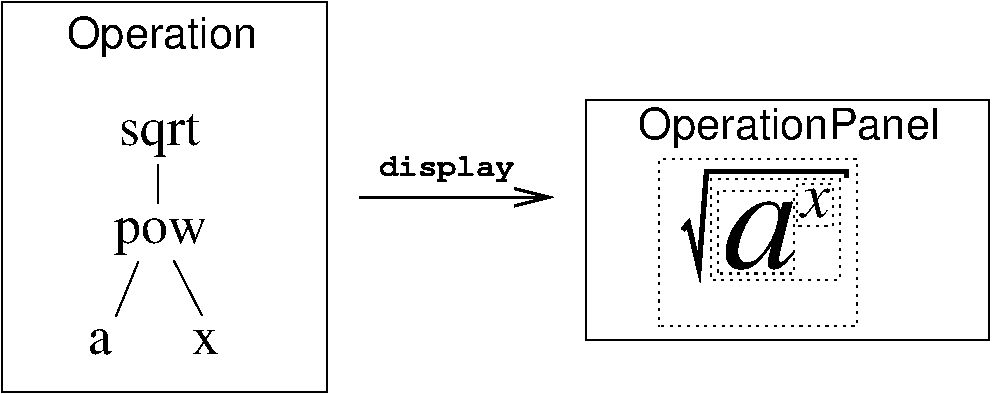
\includegraphics[width=6cm]{images/opView}}
  \hspace{1.0cm}
  \subfloat[Relations]{\label{fig:relView}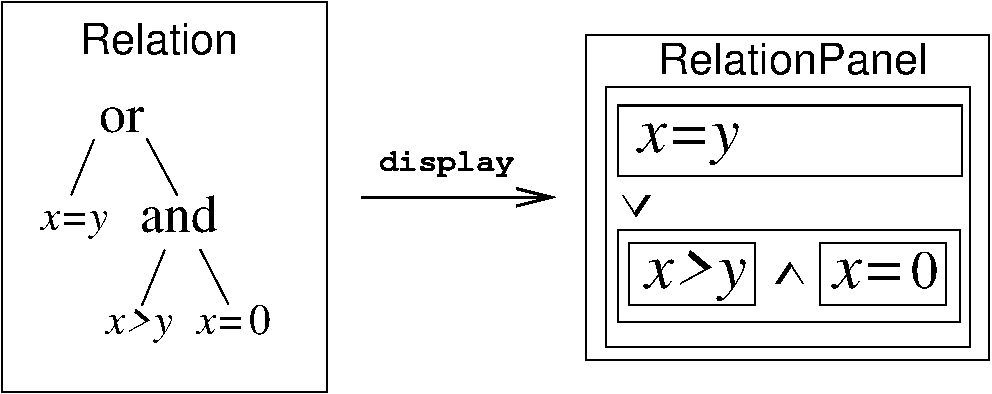
\includegraphics[width=6cm]{images/relView}}
  \caption{View architecture of algebraic expressions \cite{paehler}}
\end{figure}


\newpage

\subsection{Geometric Model}

Though the \mf supports different geometries, only affine geometric objects are implemented until now, using
however homogenous coordinates internally.
These entities allow calculations and transformations in well defined spaces and offer possibilities 
to visualize and change them both graphically and symbolically.

\subsubsection*{Geometric Groups}

As the fundament for every of its geometries, the \mf uses abstract \textit{geometric groups} for which
group operations must be defined (basically the composition). Implementations already exist for \textit{affine}
group elements and cover vector spaces, points, lines, polygons, angles, \ldots \\
Each affine group element implements the generic interface \codename{AffineGeometryIF}, extending the abstract
geometric group interface \codename{GroupElementIF}.

\subsubsection*{Affine Spaces}

As the fundament of all affine geometric objects, the entity \codename{AffineSpace} represents an affine space 
with a finite \textit{internal dimension} living in an environmental space with a finite \textit{external dimension}.
Thus a point in the $\mathbb{R}^2$ can be considered as an affine space with an internal dimension of zero
and external dimension of 2, a line with an internal dimension of one and so on. In an analogous manner,
every affine geometric entity in the \mf is integrated as an affine geometry group element.

\subsubsection*{Projective Coordinates}

In most Computer Aided Geometry (CAG) modelling software, all internal data is stored in homogenous
(i.e. \textit{projective}) coordinates, simplifying calculations in affine transformations.
Therefore every \codename{AffineSpace} uses projective coordinates internally and performs its actual 
computations in a \textit{projective space}, represented by \codename{ProjectiveSpace}. This entity uses
internally a \codename{NumberVectorSpace} with higher both internal and external dimensions and offers 
methods for working with both affine \textit{and} projective coordinates.


\vspace{0.3cm}

\subsection{Vector Space Model}

Since calculations in linear spaces of higher dimension play an important role in mathematics, the \mf 
defines a complete vector space model based on its arithmetic and geometric models and allowing to apply affine 
transformations from \textit{domain} to \textit{range} vector spaces by using the advantages of projective 
geometry.

\subsubsection*{Matrices and Tuples}

Multidimensional number computations are thereby performed by instances of \codename{NumberMatrix},
a fundamental entity in this vector space model with an own MM-implementation for e.g. visualizing and
editing arbitrary $m\times n$ number matrices. As a special extension for $m\times 1$ matrices, the
entity \codename{NumberTuple} is widely used for (vector) coordinates and matrix columns/rows, thus 
allowing to define additional features as calculating the norm or the dot product of vectors.

\subsubsection*{Basis Vectors}

Each number vector (represented by \codename{NumberVector}) is associated to a specific \codename{NumberVectorSpace}, 
defining itself a basis and which the vector's coordinates are relative to. Thus changing the basis 
of a vector space allows to transform every vector contained in it.
In order to visualize and edit both graphically and symbolically a vector space by its basis vectors, 
many MM-implementations (such as \codename{MMDefaultRN} representing the $\mathbb{R}^n$) use this 
vector space entity.

\subsubsection*{Linear Transformations}

Linear transformations or \textit{linear maps} can either be expressed by their underlying map or by 
the definition of the vector spaces they connect. In the \mf the entity \codename{LinearMap} can be used
for this purpose, allowing to apply a linear map to a \codename{NumberVector}. It uses internally instances
of \codename{NumberVectorSpace} for representing the \textit{domain} and \textit{range} vector spaces and stores
its internal matrix representation into a \codename{NumberMatrix}.\\

\begin{figure}[h!]
  \centering
  \subfloat[Domain vector space]{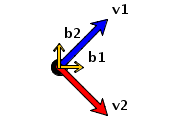
\includegraphics[scale=0.7]{images/linMap1}}
  \hspace{0.0cm}
  \subfloat[Range vector space]{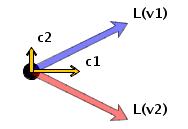
\includegraphics[scale=0.7]{images/linMap2}}
  \hspace{0.0cm}
  \subfloat[Symbolic view]{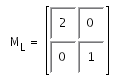
\includegraphics[scale=0.8]{images/linMap3}}
  \caption{Graphical and symbolic views of a linear map and two vectors}
  \label{fig:linMap}
\end{figure}

Again MM-implementations (such as \codename{MMDefaultRNEndomorphism} representing an endomorphism in $\mathbb{R}^n$)
exist and allow the visualization and editing of e.g. the map itself or the basis vectors of a vector space
(cf. figure \ref{fig:linMap}).



%\subsection{Graphical Views}
%\subsection{Symbolic Views}

%\newpage

%\section{Extension Framework}

%\subsection{Commom Property Format}

%\subsection{Library Extensions}

%\subsection{Mathlet Extensions}
%adaptive individual settings for mathlets


\newpage

\section{Homework Architecture}

The \mumie uses the powerful capabilities of the \mf to load, edit and save complex homework data with mathlets and
to correct and evaluate these with specialised \textit{correctors}.\\
``Saving an exercise'' means loading up the user's answers to the \mumie server and getting a \textit{receipt}
for this saving transaction.

\subsection{System Overview}

The life cycle of every homework problem consists of basically three steps:
\begin{itemize}
\item the generation of a \textit{data sheet} containing problem relevant, personalized data and
already saved answers
\item the execution of an exercise mathlet allowing to edit the answers
\item the execution of an exercise corrector evaluating the answers
\end{itemize}

Whereas the mathlet runs on the client computer inside a Java Plug-In, the first and the last steps are
executed on the server. The data exchange between the client and the \name{JAPS} server is done through 
a connection client (called \name{JapsClient}) using the \mumie common XML data format (\name{DataSheet}).


\subsubsection*{Exercise Mathlets}

A mathlet loads the problem data and already saved answers from a \mumie server (called \name{JAPS} -- Java Application Server)
and displays the values which also can be edited through this interface. Furthermore it allows to save
newer answers to the \mumie database.\\
See figure \ref{img:exercise_mathlets} for an overview of the exercise architecture in mathlets.

\begin{figure}[h]
  \begin{center}
    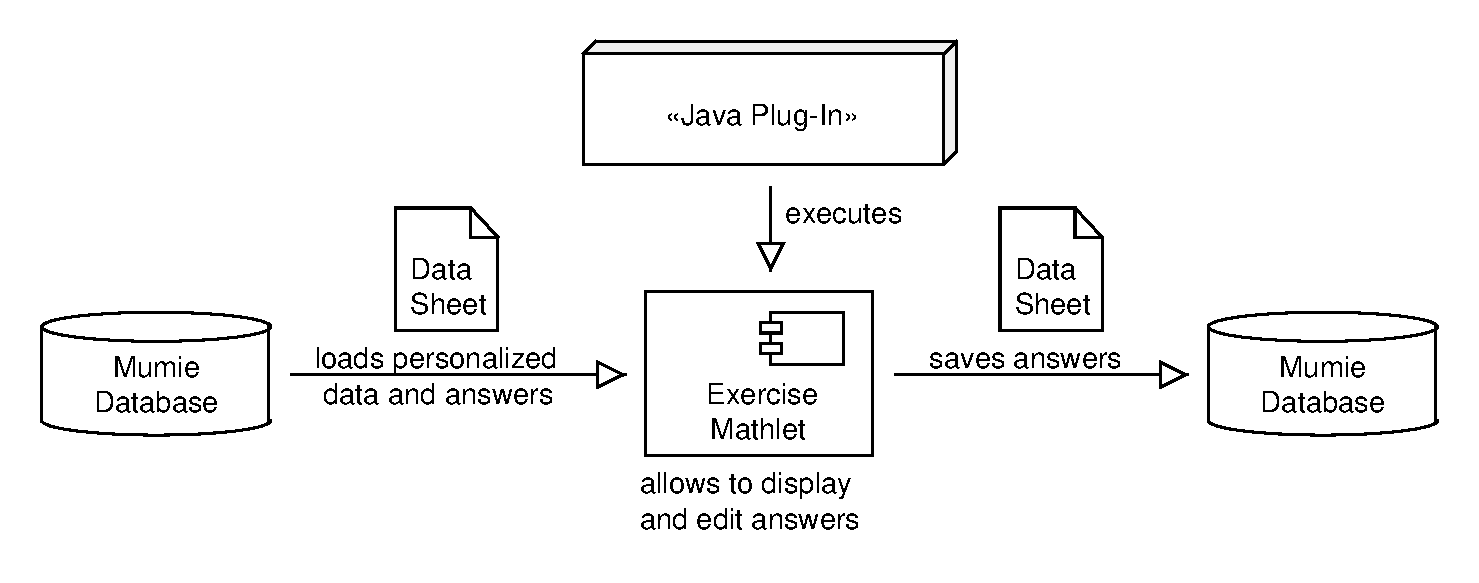
\includegraphics[width=12cm]
      {images/exercises_mathlets.pdf}
    \caption{Exercise architecture in mathlets}
    \label{img:exercise_mathlets}
  \end{center}
\end{figure}


\subsubsection*{Exercise Correctors}

A corrector will be executed on the \mumie server and allows an individual real-time ``correction'' with arbitrary complexness.
They contain individual built-in algorithms and allow the donation for correct or particulary correct answers.\\
See figure \ref{img:exercise_correctors} for an overview of the exercise architecture in correctors.


\begin{figure}[h]
  \begin{center}
    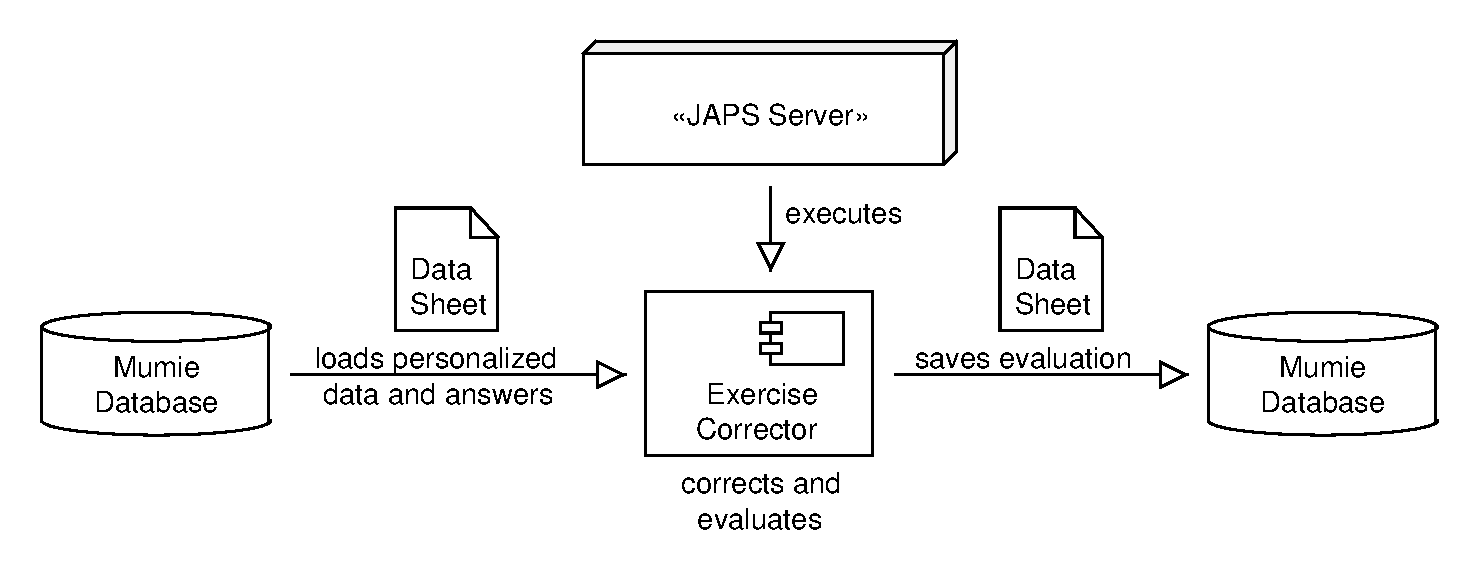
\includegraphics[width=12cm]
      {images/exercises_correctors.pdf}
    \caption{Exercise architecture in correctors}
    \label{img:exercise_correctors}
  \end{center}
\end{figure}


\subsection{Homework Receipts}

In order to have a ``record'' of the saved answers, the \mumie server returns a \textit{receipt} after the
transmission, which includes a reference to the current problem and the answers encoded in MathML.
These receipts can be used to view ``offline'' already saved answers on the server and to
give a certainty about the correlation between the entered data and that on the server.\\
An included receipt viewer allows to generically view a receipt.


\newpage

\section{Outlook}

In order to solve numerically e.g. even complex differential equations, a prospective objective is the
connection to a Computer Aided System (CAS) for numerical evaluations which require a larger computing power
or more sophisticated algorithms.\\
\\
Another primary target is the development of powerful authoring tools which shall reduce the development and 
maintenance time for mathlets/correctors while increasing quality and compatibility. A first prototype based 
on the Java development environment \oorange is available and allows an interactive and object oriented 
programming in a WYSIWYG manner of \mumie mathlets and correctors, also known as \textit{rapid prototyping}.\\
\\
A further ambitious feature is the possibility to ``script'' exercise mathlets by defining the
necessary algorithms for each problem without any knowledge about programming languages. This technique
allows the simple creation of generic homework problems while using the capabilities of the \mf in
computing, visualizing and querying mathematical content. It is intended for problems whose complexity
surpasses the possibilities of multiple choice exercises.\\
\\
A last complex endeavour is the automatical generation of meta information and thus the semantical description
of a mathematical program out of the compososition of its components. This necessitates the design of an
appropriate meta language, able to describe the ontology of mathematical problems, and the development of
identification pattern for mapping mathematical entities and their relationships onto semantic structures.


\begin{thebibliography}{9}
 
\bibitem{paehler}
  Dr. Tim Paehler,
  \emph{Design, Implementation and Application of a Reusable Component Framework for Interactive
  Mathematical eLearning Sites}.
  Dissertation, RWTH Aachen,
  March 2005.
 
\bibitem{sun1}
  Sun Microsystems, Inc.,~
  \emph{Java Plugin Guide}.~ \texttt{\url{http://java.sun.com/j2se/1.5.0/docs/guide/plugin/developer_guide/contents.html}}.
 
\bibitem{sun2}
  Sun Microsystems, Inc.,
  \emph{Java Deployment Guide}. \texttt{\url{http://java.sun.com/j2se/1.5.0/docs/guide/deployment/deployment-guide/contents.html}}.
 
\bibitem{sun3}
  Sun Microsystems, Inc.,
  \emph{The Swing Tutorial}. \texttt{\url{http://java.sun.com/docs/books/tutorial/uiswing/index.html}}.
 
\end{thebibliography}

\end{document}
